\chapter{Konzeption}
\label{chapter:Konzeption}

\section{Konzeption der Anwendung} %Benedikt
\label{section:Konzeption der Anwendung} %Benedikt
<<Benedikt>>

\subsection{Grundidee} %Benedikt
\label{subsection:Grundidee} %Benedikt
<<Benedikt>>

\subsection{Mockup} %Benedikt
\label{subsection:Mockup} %Benedikt
<<Benedikt>>

\subsection{Das Neuroph Framework} %Benedikt
\label{subsection:Das Neuroph Framework} %Benedikt
<<Benedikt>>

\section{Konzeption des künstlichen neuronalen Netzes}
\label{section:Konzeption des künstlichen neuronalen Netzes}

In den folgenden Abschnitten wird ein \acs{knn} konzeptioniert, dass als Vorlage für alle zu erstellenden \acs{knn} zur Prognose von Börsenkursen dienen soll. 

\subsection{Wahl des Netztyps}
\label{subsection:Wahl des Netztyps}
Zunächst ist zu ermitteln, welche Netztypen sich zur Prognose von Börsenkursen grundsätzlich eignen. Nicht jeder Netztyp ist gleichermaßen zur Prognose geeignet. Bestimmte \acs{knn} sind beispielsweise überhaupt nicht in der Lage, Prognosen zu erstellen. 

Grundsätzlich lassen sich \acs{knn} in zwei Oberklassen unterteilen. Es gibt hetero-assoziative Netze sowie die auto-assoziative Netze. Hetero-assoziative Netze bilden einen Vektor $A$ der Länge $n$ auf einem Vektor $B$ einer meist kürzeren Länge $m$ $\{m \in \mathbb{N} | m \le n\}$ ab. Auto-assoziative Netze wiederum bilden einen Eingabevektor der Länge $n$ auf einem Ausgabevektor der gleichen Länge ab. Innerhalb dieser zwei Klassen lassen sich \acs{knn} wiederum in mehrere Netztypen aufteilen. Die folgende Tabelle liefert hierzu eine Übersicht:

\begin{center}
\begin{tabular}{|c|c|}
\hline 
\textbf{Hetero-assoziative Netzmodelle} & \textbf{Auto-assoziative Netzmodelle} \\ 
\hline 
(M)Adaline & Hopfield-Netze \\ 
\hline  
Perzeptron &  Boltzmann Maschinen \\ 
\hline 
Multilayerperzeptron & - \\ 
\hline 
\end{tabular} 
\end{center}

Das \acs{knn} soll mithilfe von mehreren vorhergehenden Börsenkursen den zukünftigen Börsenkurs prognostizieren. Da es sich bei den zu prognostizierenden Börsenkurs um einen skalaren Wert handelt, ist die Anzahl der Eingabeneuronen (und damit die Anzahl der Elemente des Eingabevektors) höher als die Anzahl der Ausgabeneuronen (und damit höher als die Anzahl der Elemente des Ausgabevektors). Somit sind für diese Seminararbeit nur hetero-assoziative Netze von Relevanz.

Aus der Menge der hetero-assoziativen Netze ist nun der Netztyp zu ermitteln, der für die Anwendung am geeignetsten ist.

Zur Wahl eines geeigneten Netztyps kann zunächst die Lineare Separierbarkeit betrachtet werden:

\newmdtheoremenv{defi}{Definition}
\begin{defi}Definition der linearen Separierbarkeit\\
Seien $X_{0}$ and $X_{1}$ zwei Datenmengen im $n$-dimensionalen euklidischen Raum. Dann sind die Mengen $X_{0}$ and $X_{1}$ genau dann  "`linear separierbar"', wenn es  $n+1$ Werte $w_{1}, w_{2},..,w_{n}, k$, gibt, sodass jeder Punkt  $x \in X_{0}$ die Bedingung $\sum^{n}_{i=1} w_{i}x_{i} > k$ erfüllt und jeder Punkt $x \in X_{1}$ die Bedingung $\sum^{n}_{i=1} w_{i}x_{i} < k$ erfüllt.
\end{defi}

Um das Verständnis der oben genannten Definition zu erleichtern, kann die folgende Abbildung betrachtet werden:

\begin{figure}[H]
\centering
		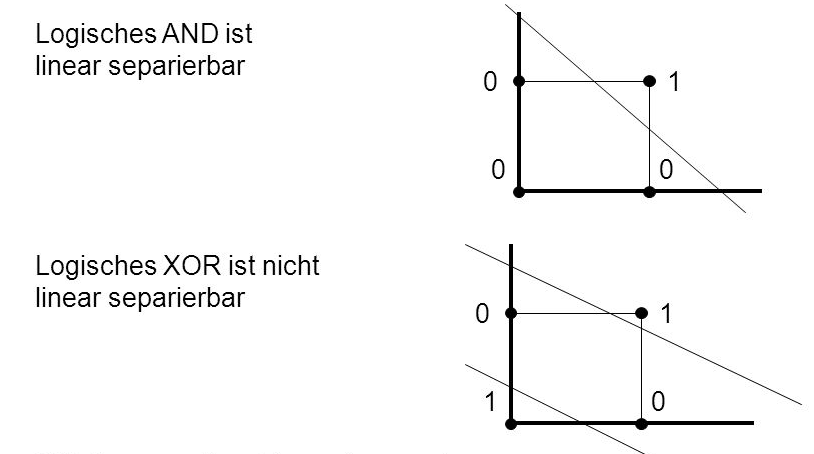
\includegraphics[width=0.95\textwidth]{Linear_Sep.PNG}
	\caption{Bildliche Erläuterung der linearen Separierbarkeit}
	\label{fig:Bildliche Erläuterung der linearen Separierbarkeit}
\end{figure}

Man erkennt also, das eine zweidimensionale Funktion dann als linear separierbar gilt, wenn zwischen zwei Ergebnismengen der Funktion eine Gerade gelegt werden kann. Analog setzt sich dies in Funktionen höherer Dimensionen fort. Ist die Funktion zum Beispiel dreidimensional, erfolgt die Separierung durch eine Ebene.

Es ist bewiesen, dass einschichtige \acs{knn} nur in der Lage sind, linear separierbare Funktionen zu berechnen. Den Konkreten Beweis dazu liefern Minski \& Papert am Beispiel des XOR-Problems:

\newmdtheoremenv{bew}{Beweis}
\begin{bew}Beweis der Eingeschränkten Fähigkeit von KNN anhand des XOR-Problems\\

Gegeben sind:\\

Ein Perzetron der folgenden Bauart:

\begin{figure}[H]
\centering
		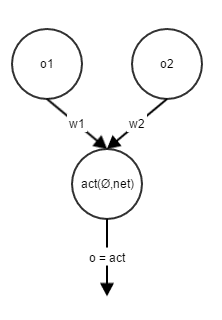
\includegraphics[width=0.20\textwidth]{Perzeptron.PNG}
	\caption{Beispielperzeptron zur Darstellung des XOR-Problems}
	\label{fig:Beispielperzeptron zur Darstellung des XOR-Problems}
\end{figure}

und folgende Rahmenbedingungen:

$w_1\cdot1 + w_2\cdot2 = net$\\ 
$f_(act)(o) = id$ \\
$\emptyset = Schwellenwert$

Dann gilt folgendes:\\
$a) w_1\cdot0 + w_2\cdot0 \le \emptyset$ Bei einem Inputvektor (0,0) liefert der Output 0.\\
$b) w_1\cdot0 + w_2\cdot0 \geq \emptyset$ Bei einem Inputvektor (0,1) liefert der Output 1.\\
$c) w_1\cdot0 + w_2\cdot0 \geq \emptyset$ Bei einem Inputvektor (1,0) liefert der Output 1.\\
$d) w_1\cdot0 + w_2\cdot0 \le \emptyset$ Bei einem Inputvektor (1,1) liefert der Output 0.\\

Der Widerspruch ergibt sich wie folgt:\\ $(b+c):  w_1 + w_2 \geq \emptyset  \wedge (d)  w_1 + w_2 \leq \emptyset$
\end{bew}

Dieser Beweis kann ebenfalls auf andere nicht linear separierbare Funktionen angewandt werden.Somit steht fest, dass ein einschichtiges Perzeptron nicht in der Lage sein kann, nicht linear separierbare Funktionen zu approximieren.

Auf Basis der oben genannten Tatsache kann ermittelt werden, ob ein einschichtiges Perzeptron zur Approximation von Börsenkursen geeignet ist. Dafür wurde ein ein Perzeptron folgender Bauart entwickelt und untersucht, ob dieses Konvergiert.

\begin{figure}[H]
\centering
		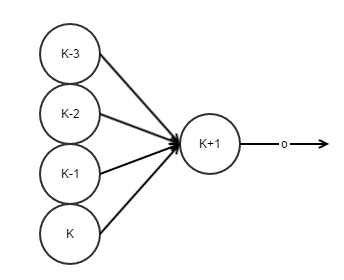
\includegraphics[width=0.5\textwidth]{Testperzeptron.PNG}
	\caption{Grundlegendes Konzept des KNN}
	\label{fig:Grundlegendes Konzept des KNN}
\end{figure}

Bei Betrachtung des Netzwerkfehlers des Perzeptrons erkennt man, dass das Perzeptron nicht konvergiert:

\begin{figure}[H]
\centering
		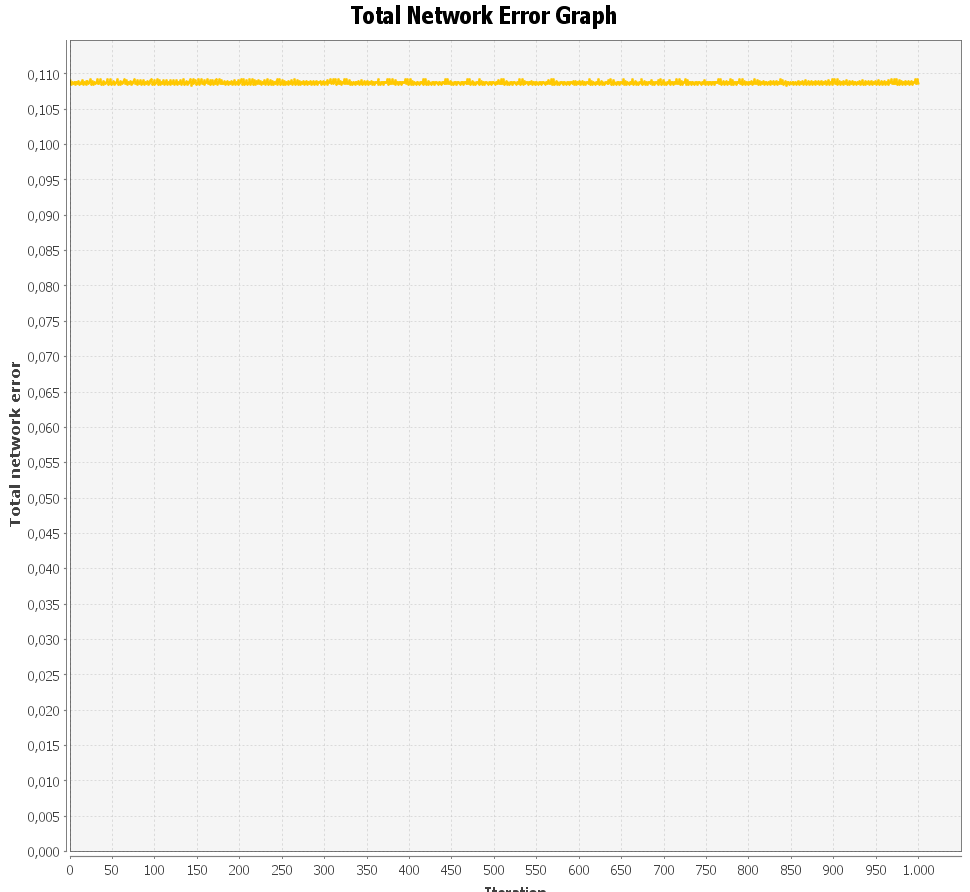
\includegraphics[width=0.5\textwidth]{MSEperzeptron.PNG}
	\caption{Grundlegendes Konzept des KNN}
	\label{fig:Grundlegendes Konzept des KNN}
\end{figure}

Der Netzwerkfehler des Perzeptrons bleibt über alle Iterationen konstant auf einen Niveau von circa $0,10$.

Nun ist es sinnvoll, folgendes Theorem zu berücksichtigen:
 
\newmdtheoremenv{theo}{Theorem}
\begin{theo}Konvergentheorem von Rosenblatt\\
Der Lernalgorithmus des Perzeptrons konvergiert in endlicher Zeit, d.h. das Perzeptron kann in endlicher Zeit alles lernen, was es repräsentieren kann.
\end{theo}

Betrachtet man alle oben genannten mathematischen Gegebenheiten, ergibt sich die folgende Relation:

Perzeptron konvergiert $\rightarrow$ Funktion Linear separierbar $\rightarrow$ Perzeptron geeignet.
und natürlich analog:Perzeptron konvergiert nicht $\rightarrow$ Funktion nicht Linear separierbar $\rightarrow$ Perzeptron nicht geeignet.

Folglich bleibt nur noch das Multilayerperzeptron als Mögliche Auswahl übrig. Das dieses \ac{knn} tatsächlich zur Prognose geeignet ist, belegt das folgende Theorem:

\begin{theo}Theorem von Kolmogorov\\
Für ${n \in \mathbb{N} | n>2}$ lässt sich jede reellwertige Funktion $f:[0;1]^n\rightarrow[0;1]$ durch ein dreischichtiges vorwärtsverknüpftes Netz mit maximal $n$ Einheiten in der Eingabeschicht,$(2n+1)$ Einheiten in der Zwischenschicht und $2n+1$ Einheiten in der Ausgabeschicht berechnen.
\end{theo}

Ein Börsenkurs kann prinzipiell jede beliebige Funktion annehmen. Durch das obige Theorem ist jedoch sichergestellt, dass das mehrschichtige vorwärtsgerichtete Netz in der Lage ist, diese Funktionen zu approximieren, da ein Multilayerperzeptron als universeller Aprroximator fungiert.

\subsection{Wahl der Topologie}
\label{subsection:Wahl der Topologie}

Zur Prognose des Börsenkurses sollen die letzten vier Börsenkurse als Input dienen. Durch diesen Input soll der Börsenkurs am nächsten Tag prognostiziert werden. Zur richtigen Dimensionierung der inneren Schicht können einige Richtlinien berücksichtigt werden:

\begin{itemize}
\item Die Anzahl der versteckten Neuronen in der inneren Schicht sollte nicht zu groß gewählt werden, damit das Netz das antrainierte Verhalten nicht "'auswending`" lernt und dieses dann nur bereits trainierte Muster anwenden kann und es somit die Generalisierungsfähigkeit verliert. Man spricht in diesem Fall von Overfittin.g 
\item Die Anzahl der versteckten Neuronen in der inneren Schicht sollte auch nicht zu klein gewählt werden, da eine gewisse Menge an Neuronen wichtig sind, um sich Regeln merken zu können.
\item Eine grobe Annäherung zur Bestimmung der Obergrenze der Anzahl von Neuronen in der versteckten Schicht liefert die folgende Formel:

\begin{equation}\formelentry{Optimale Anzahl Neuronen in der versteckten Schicht}
  N_h = \frac{N_d}{10*(N_i+N_o)}
\end{equation}
Nh ist hierbei die Obergranze, Ni ist die Anzahl der Inputneuronen und No die Anzahl der Outputneutonen. Da 450 Trainingsdaten verwendet werden. Bedeutet das für diese SEminararbeit konkret:

\begin{equation}\formelentry{Optimale Anzahl Neuronen in der versteckten Schicht}
  N_h = \frac{450}{10*(4+1) = 9 }   
\end{equation}
\end{itemize}
 

Somit ergibt sich insgesamt die folgende Topoologie:

\begin{figure}[H]
\centering
		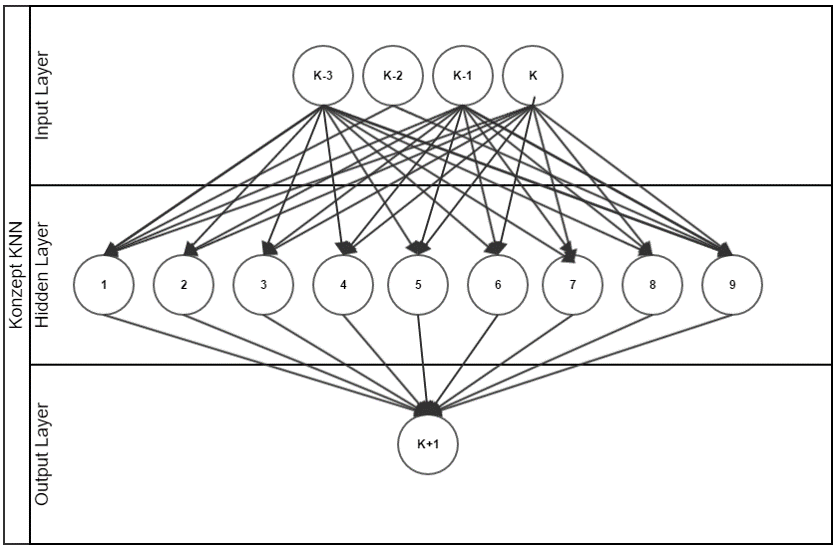
\includegraphics[width=0.5\textwidth]{KonzKNN.PNG}
	\caption{Grundlegendes Konzept des KNN}
	\label{fig:Grundlegendes Konzept des KNN}
\end{figure}


Die oben abgebildete Topologie stellt ein solides Grundkonstrukt dar, das in der Umsetzungsphase noch weiter optimiert werden kann.


\subsection{Wahl des Lernverfahrens} 
\label{subsection:Wahl des Lernverfahrens}

Grundsätzlich gibt es drei grobe Klassifikation von Lernverfahren. in diesem Abschnitt werden alle drei Lernverfahren näher vorgestellt und anschließend eine Begründete Auswahl der Lernverfahrens getroffen.

\begin{itemize}
\item Überwachtes Lernen: Beim überwachten Lernen sind sowohl die Eingabedaten sowie die dazugehörigen Ausgabedaten bekannt. Mit Hilfe dieser Daten kann das \ac{knn} dann trainiert werden. Die berechneten Ausgabedaten können anschließend mit den tatsächlichen Ausgabedaten verglichen werden. Dieser Fehler wird dann genutzt, um die Verbindungsgewichte des \ac{knn} anzupassen. Typische Vertreter dieses Lernverfahrens sind die sogenannten Backpropagation-Lernverfahren.
	
\item Bestärkendes Lernen
Ähnlich wie das überwachte Lernen, jedoch biologisch motivierter ist  das sogenannte bestärkende Lernen. Hier sind dem \ac{knn} die Eingabewerte zwar bekannt, aber die dazugehörigen Ausgabewerte nur zum Teil oder gar nicht. Das \ac{knn} wird lediglich darüber informiert, das Ergebnis richtig bzw. falsch war. Es ist ein sehr Zeitaufwändiges Lernverfahren, da es die Gewichte auf Grund der spärlichen Information nur sehr langsam anpassen kann. Dieser Verfahren kann als Mischung aus überwachtes Lernen und unüberwachtes Lernen gesehen werden.

\item Unüberwachtes Lernen
Das unüberwachte Lernen ist biologisch gesehen am plausibelsten. Bei diesem  Lernverfahren besteht existieren nur Eingabemuster, es existieren keine erwünschten Ausgaben oder Angaben, ob das Netz die Eingaben richtig oder falsch klassifiziert hat. Stattdessen versucht der Lernalgorithmus selbständig, Gruppen ähnlicher Eingabevektoren zu identifizieren und diese auf Gruppen ähnlicher oder benachbarter Neuronen abzubilden. 
\end{itemize}


Da sowohl die Eingabewerte als auch die Ausgabewerte der zu verwendenden Datensätze bekannt sind, bietet sich das überwachte Lernen an. Verglichen mit den anderen Lernverfahren ist dies die effizienteste Lernmethode. Sie verfügt zwar über kein biologisches Vorbild, dieser Umstand hat aber für diese Seminararbeit keine Relevanz.

